\documentclass{beamer}

\usepackage[english]{babel}
\usepackage{multirow}
\usepackage{amsmath}
\usepackage{amsfonts}
\usepackage{xkeyval}
\usepackage{graphics}
\usepackage{url}
\usepackage{cases}
\usepackage[lined,boxed,linesnumbered]{algorithm2e}

\definecolor{mycolor}{RGB}{220,20,29}
\definecolor{mycolorlys}{RGB}{214,45,56}
\definecolor{mycolorlyslys}{RGB}{200,57,58}
\definecolor{mycolorlyslyslys}{RGB}{190,96,94}
%\mode<presentation>
%{
  %\usetheme{}
  %\usecolortheme{beaver}
  % 可供选择的主题参见 beameruserguide.pdf, 第 134 页起
  % 无导航条的主题: Bergen, Boadilla, Madrid, Pittsburgh, Rochester;
  % 有树形导航条的主题: Antibes, JuanLesPins, Montpellier;
  % 有目录竖条的主题: Berkeley, PaloAlto, Goettingen, Marburg, Hannover;
  % 有圆点导航条的主题: Berlin, Dresden, Darmstadt, Frankfurt, Singapore, Szeged;
  % 有节与小节导航条的主题: Copenhagen, Luebeck, Malmos, Warsaw
  %\setbeamercovered{transparent}
  % 如果取消上一行的注解 %, 就会使得被覆盖部分变得透明(依稀可见)
%}
\mode<presentation>
{
    \usetheme{Madrid}
    \usecolortheme[named=mycolor]{structure}
    \useinnertheme{circles}
    \usefonttheme[onlymath]{serif}
    \setbeamertemplate{blocks}[rounded][shadow=true]
}

%\logo{
\includegraphics[scale=0.08]{images/HUSTLogo}}
\title{Knowledge Adaptation for Ad Hoc Multimedia Event Detection with Few Exemplars}
\subtitle{Z. Ma, Y. Yang, Y. Cai, N. Sebe and A. Hauptmann-ACM MM2012}
\author{Yunfei Wang}
\institute{Department of Computer Science \& Technology\\Huazhong University of Science \& Technology}
\date{\today}

\begin{document}

\begin{frame}
\titlepage
\end{frame}

\begin{frame}
\tableofcontents
\end{frame}

%==============================================================
\section{Basic Concepts}
\begin{frame}\frametitle{Basic Concepts}
\begin{description}
  \item[Concept] An abstract or general idea inferred from specific instances, e.g. fish,sky.
  \item[Event] An observable occurrence, e.g. making a cake,landing a fish.
  \item[Recognition] Associate objects that is already known with one or more labels.
  \item[Detection] Detect the existence of concepts or events coming from an infinite semantic space through pre-trained detectors.
  \item[Knowledge Adaptation] Also known as transfer learning, propagate knowledge from an auxiliary domain to a target domain.
\end{description}
In Ad Hoc MED,events are more generic and the events are unknown before conducting the detection task.Besides, there are few positive examples for training.
\end{frame}

\section{Video Representation}
\begin{frame}\frametitle{Illustration of framework}
\begin{figure}
  \centering
  % Requires \usepackage{graphicx}
  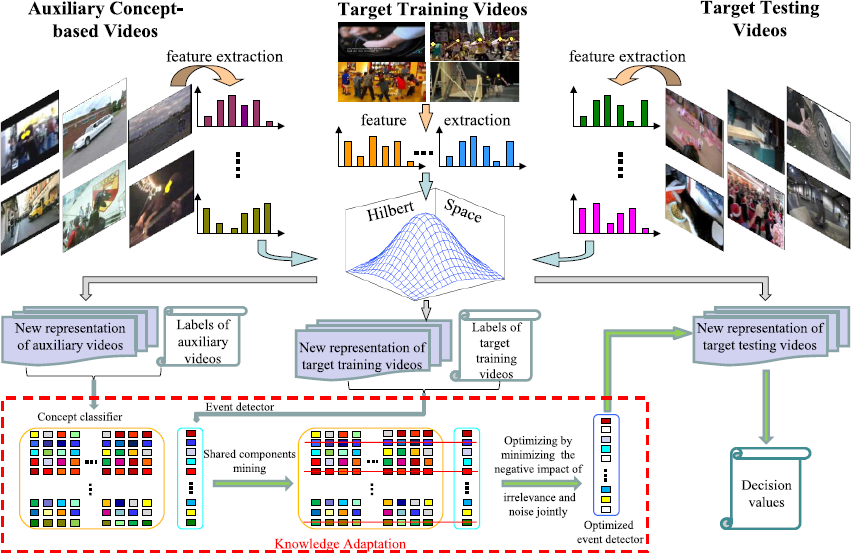
\includegraphics[scale=0.46]{images/framework}\\
  \caption{Framework}\label{pic:framework}
\end{figure}
\end{frame}

\begin{frame}\frametitle{Preprocessing each video}
\begin{exampleblock}{Procedures}
\begin{enumerate}
\item Extract \textcolor{red}{Key Frames} using shot boundary detection algorithm
\item Detect \textcolor{red}{Interest Points} utilizing Harris-Laplace interest point detector
\item Obtaining \textcolor{red}{SIFT/CIFT features}
\item Generate \textcolor{red}{Bag-of-Words feature} though clustering SIFT/CSIFT features
\item Map BoW feature into Hilbert Space with kernel trick
\item Perform full rank \textcolor{red}{Principal Component Analysis} in another Hilbert Space.
\end{enumerate}
\end{exampleblock}
\end{frame}

%==============================================================
\section{Concepts Adaptation Assisted Event Detection}
\begin{frame}\frametitle{Explore knowledge from target training videos}
$\tilde{X}_t=\{\tilde{x}_t^1,\tilde{x}_t^2,\cdots,\tilde{x}_t^{n_t}\}\in\mathbb{R}^{d_h\times n_t}$:training videos in Hilbert Space\;\\
$y_t=\{y_t^1,y_t^2,\cdots,y_t^{n_t}\}^T\in\{0,1\}^{n_t\times 1}$:corresponding labels.
\begin{block}{}
Associate low-level representations and high-level semantics of videos by a decision function $f$:
\begin{equation}\label{eq:decisionfun}
f_t(\tilde{X}_t)=\tilde{X}_t^TW_t+1_tb_t
\end{equation}
where $W_t\in\mathbb{R}^{d_h\times 1}$ is an event detector which correlates $\tilde{X}_t$ with labels $y_t$.
\end{block}

\begin{block}{}
$f_t$ is decided by minimizing the following objective:
\begin{equation}\label{eq:decidef}
\min_{f_t} loss(f_t(X_t),y_t)+\mu\Omega(f_t)
\end{equation}
\end{block}

\begin{block}{}
Using $l_{2,1}$-norm based loss function because it's robust to outliers.Reformulate Eq.(\ref{eq:obj1}):
\begin{equation}\label{eq:obj1}
\min_{W_t,b_t}\left\Vert{{X}_t^TW_t+1_tb_t-y_t}\right\Vert_{2,1}+\mu\Omega(W_t)
\end{equation}
\end{block}
\end{frame}

\begin{frame}\frametitle{Adapt knowledge from auxiliary videos}
$\tilde{X}_a=\{\tilde{x}_a^1,\tilde{x}_a^2,\cdots,\tilde{x}_a^{n_a}\}\in\mathbb{R}^{d_h\times n_a}$:auxiliary videos.\\
$Y_a=\{y_a^1,y_a^2,\cdots,y_a^{n_a}\}^T\in\{0,1\}^{n_a\times c_a}$:label matrix.
\begin{block}{}
Mine the correlation between low-level representations and high-level semantics of the auxiliary concepts-based videos.
\begin{equation}\label{eq:obj2}
\min_{W_a,b_a}\left\Vert \tilde{X}_a^TW_a+1_ab_a-Y_a\right\Vert_{2,1}+\gamma\Omega(W_a)
\end{equation}
where $W_a\in\mathbb{R}^{d_h\times c_a}$ is a concept classifier.
\end{block}
\end{frame}

\begin{frame}\frametitle{Bridge the gap between concepts and event}
\begin{enumerate}
\item Knowledge adaptation is based on the assumption that there are shared structures between the source and the target.
\item The shared noisy and irrelevant components in video representation weaken the performance of event detector.So they must be removed.
\item Concepts of $\tilde{X}_a$ and events of $\tilde{X}_t$ are related and grounded on similar low-level representations by $W_a$ and $W_t$ respectively.So the irrelevant or noisy components is similar in $W_a$ and $W_t$,which can be uncovered by learning $W_a$ and $W_t$ jointly.
\end{enumerate}
\end{frame}

\begin{frame}\frametitle{Objective function}
\begin{block}{Joint information}
event detector:$W_t=\left[ w_t^1,w_t^2,\cdots,w_t^{d_h}\right]$\\
concept classifier:$W_a=\left[ w_a^1,w_a^2,\cdots,w_a^{d_h}\right]$\\
joint analyzer:$W=\left[ w^1,w^2,\cdots,w^{d_h}\right]$,reflecting joint information from auxiliary videos and training videos,where $w^i=[w_a^i,w_t^i]$.
\end{block}
\begin{block}{Remove shared irrelevant and noisy components using sparse model}
$\min\left\Vert W\right\Vert_{2,p}=\left(\sum_{i=1}^{d_h}\left(\sum_{j=1}^{c_a+1} W_{ij}^2 \right)^{\frac{1}{2}}\right)^{2-p}$
\end{block}
\begin{block}{Final objective function}
$\min_{W_a,W_t,b_a,b_t}\left\Vert \tilde{X}_a^TW_a+1_ab_a-Y_a\right\Vert_{2,1}+\left\Vert \tilde{X}_t^TW_t+1_tb_t-y_t\right\Vert_{2,1}+\alpha\left(\sum_{i=1}^{d_h}\left(\sum_{j=1}^{c_a+1}\vert W_{ij}\vert\right)^{\frac{p}{2}}\right)^{\frac{1}{p}}+\beta\left(\Vert W_a\Vert_F^2+\Vert W_t\Vert_F^2\right)$
\end{block}
\end{frame}

%===============================================================
\section{Optimizing the Event Detector}
\begin{frame}\frametitle{Algorithm}
\begin{algorithm}[H]
\KwIn{Auxiliary data $\tilde{X_a}\in\mathbb{R}^{d_h\times n_a},Y_a\in\mathbb{R}^{n_a\times c_a}$\;
Training data $\tilde{X_t}\in\mathbb{R}^{d_h\times n_t},y_t\in\mathbb{R}^{n_t\times 1};$ Parameters $\alpha$,$\beta$.}
\KwOut{Optimized $W_t\in\mathbb{R}^{d_h\times 1}$ and $b_t\in\mathbb{R}^1$.}

Set $t=0$,initialize $W_a\in\mathbb{R}^{d_h\times c_a}$ and $W_t\in\mathbb{R}^{d_h\times 1}$ randomly\;

\Repeat{Convergence}{
Compute $\tilde{X}_a^TW_a+1_ab_a-Y_a=\left[u^1,\cdots,u^{n_a}\right]^T,\tilde{X}_t^TW_t+1_tb_t-y_t=\left[v^1,\cdots,v^{n_t}\right]^T$,and $W=\left[w^1,\cdots,w^d\right]^T$\;
$D_a^{ii}=\frac{1}{2\|u^i\|_2}$,$D_t^{ii}=\frac{1}{2\|v^i\|_2}$,and $D^{ii}=\frac{1}{\frac{2}{p}\|w^i\|_2^{2-p}}$\;
$W_a^{t+1}=(\tilde{X}_aH_aD_aH_a\tilde{X}_a^T+\alpha D+\beta I_d)^{-1}\tilde{X}_aH_aD_aH_aY_a$\;
$b_a^{t+1}=\frac{1}{n_a}1_a^TY_a-\frac{1}{n_a}1_a^T\tilde{X}_a^TW_a^{t+1}$\;
$W_t^{t+1}=(\tilde{X}_tH_tD_tH_t\tilde{X}_t^T+\alpha D+\beta I_d)^{-1}\tilde{X}_tH_tD_tH_ty_t$\;
$b_t^{t+1}=\frac{1}{n_t}1_t^Ty_t-\frac{1}{n_t}1_t^T\tilde{X}_t^TW_t^{t+1};t=t+1$\;
}

\Return $W_t$ and $b_t$.
\caption{Optimizing the event detector}
\end{algorithm}
\end{frame}

\end{document}
